\subsection{前端设计}

\begin{figure}[H]
  \centering
  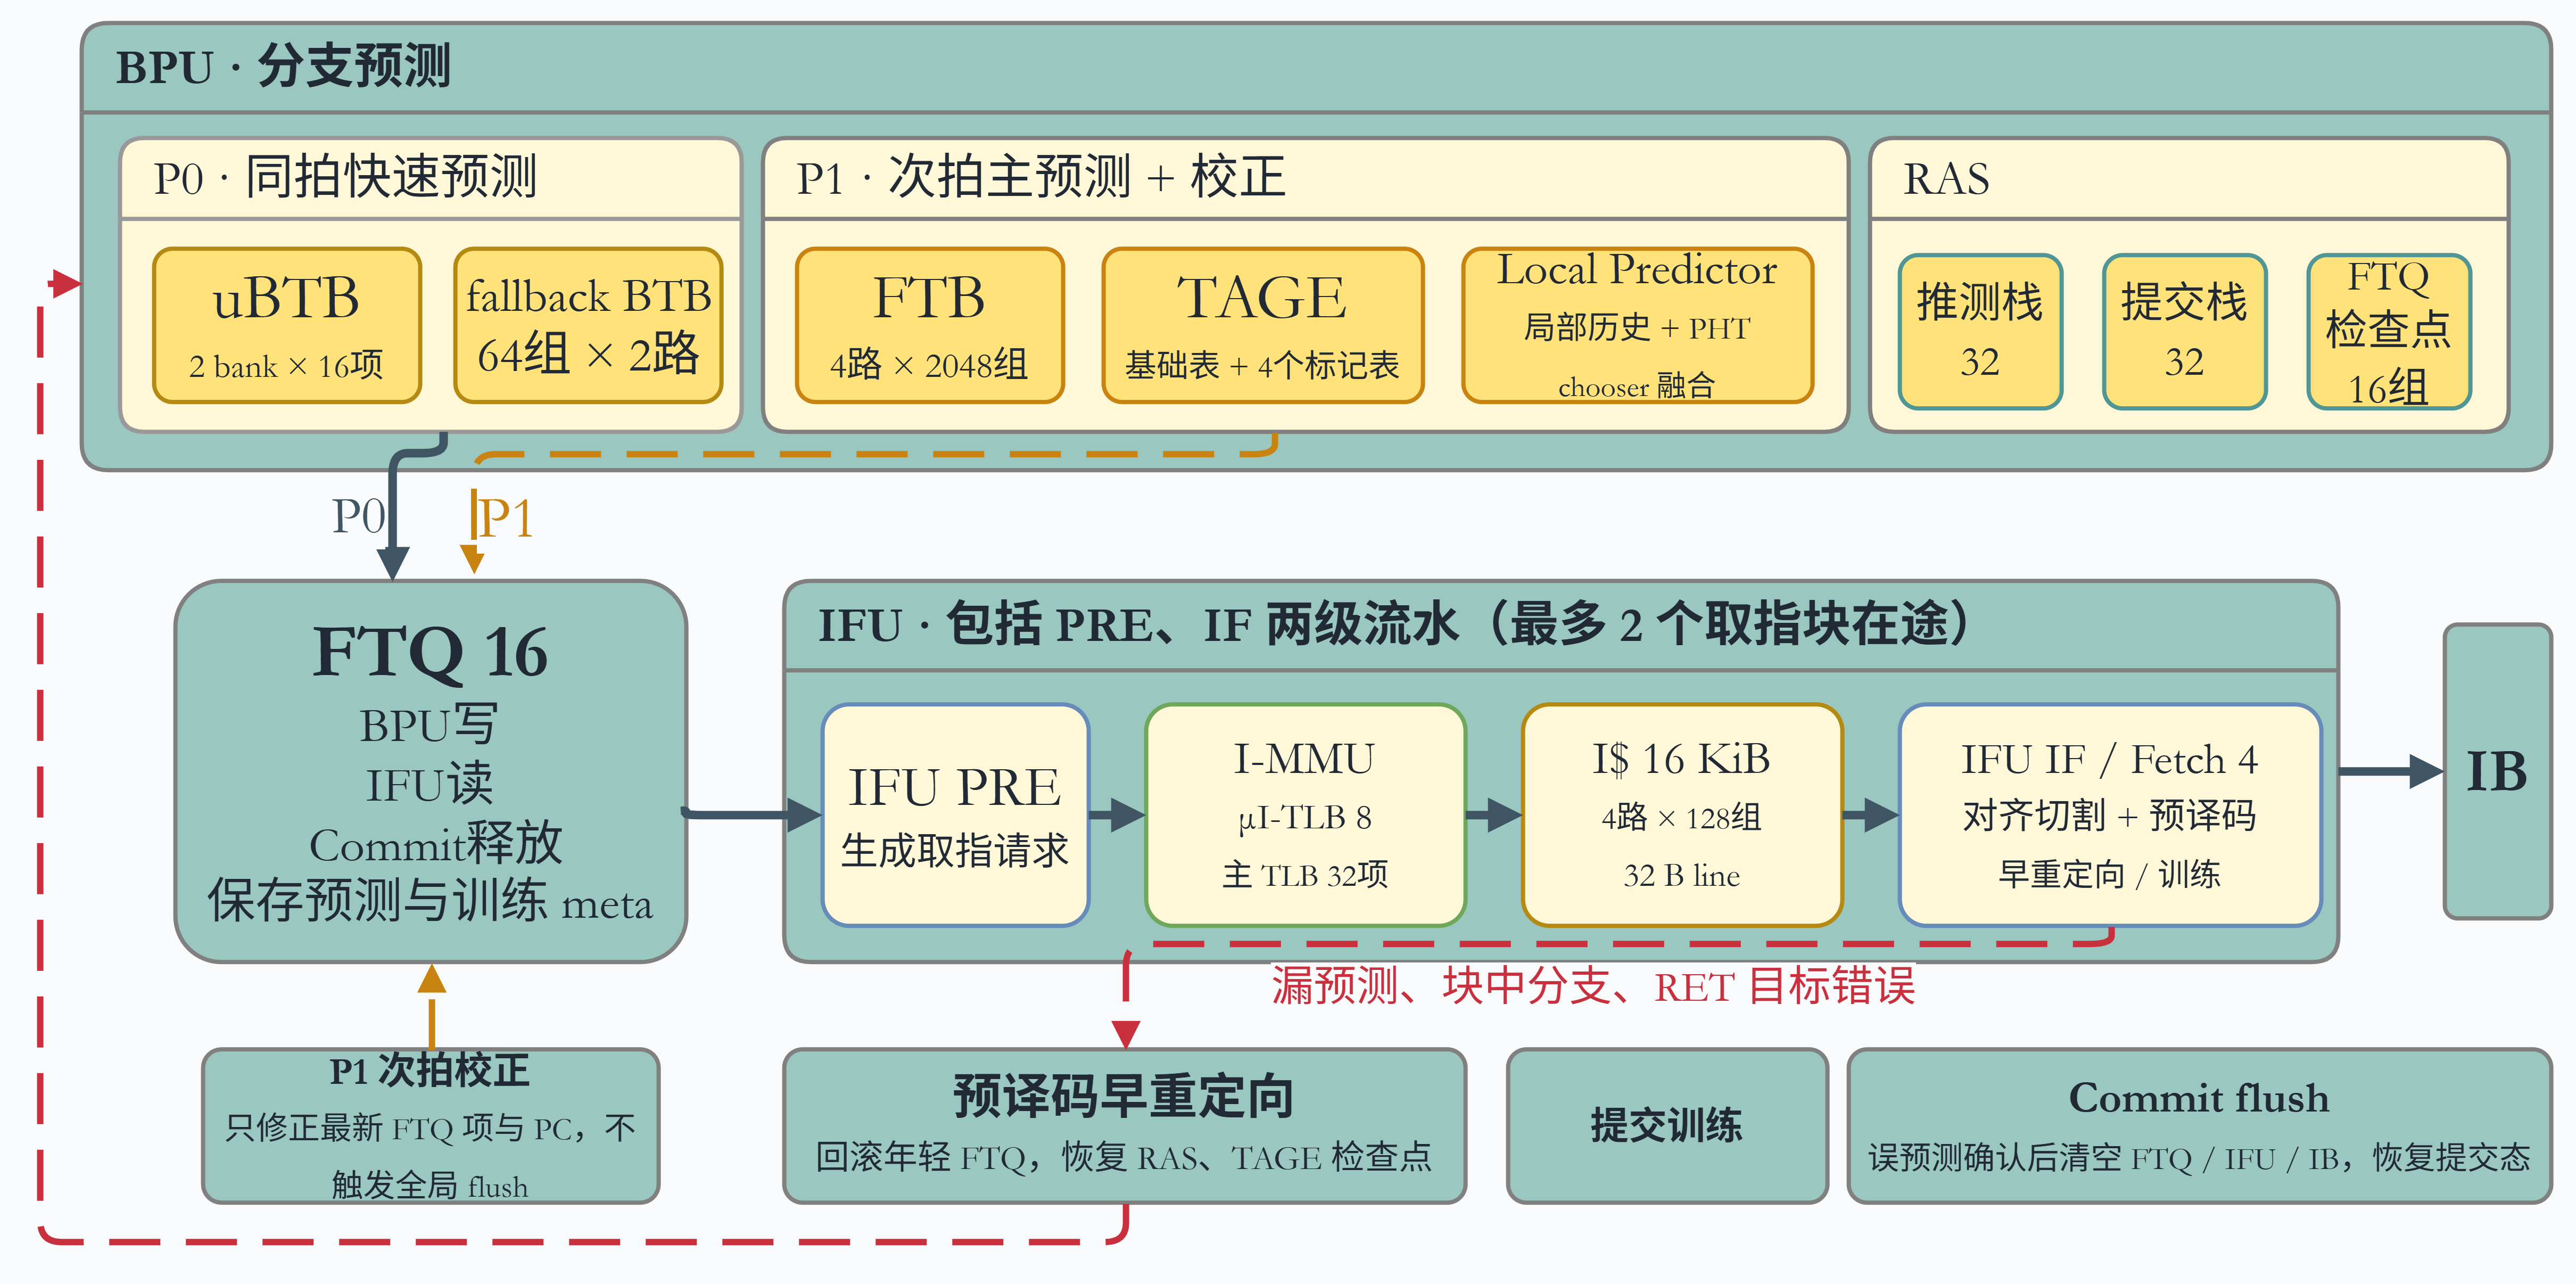
\includegraphics[width=0.95\textwidth]{figure/frontend.png}
  \caption{前端架构图}
  \label{fig:frontend}
\end{figure}

前端采用基本块取指结构，主要包含分支预测器（BPU）、取指目标队列（FTQ）、取指单元（IFU）、一级指令缓存（ICache）和指令缓冲（IB）。BPU 每拍针对一个起始 PC 产生一个预测块，块内最多包含 4 条指令，并在 4\,KB 页边界处截断，避免一次预测跨越两个地址翻译页。

\subsubsection{分支预测器}

分支预测器采用 P0/P1 两级响应。P0 使用快速结构当拍给出基线预测，P1 在下一拍返回容量更大的主预测结果；若两级结果不一致，则修正 FTQ 中对应条目并重定向前端。

\begin{itemize}
  \item \textbf{uBTB}：两银行、每银行 16 项，共 32 个物理表项；每次查询一个 16 路全相联银行，提供 P0 快速目标；
  \item \textbf{fallback BTB}：两路、每路 64 组，共 128 项，在 uBTB 未命中时提供快速后备目标；
  \item \textbf{FTB}：4 路$\times$2048 组，共 8192 项，保存基本块内分支位置、类型、目标和顺序下落地址；
  \item \textbf{TAGE}：8192 项基础计数表与 4 张各 2048 项、12 位标签的历史表，全局历史长度为 4/10/24/64；
  \item \textbf{局部预测器}：2048 项、每项 12 位的局部历史表，配合 4096 项两位计数 PHT 与选择器，补充规律性局部分支；
  \item \textbf{RAS}：32 项推测栈和 32 项提交栈组成双栈，在函数调用/返回预测与提交恢复之间隔离投机状态。
\end{itemize}

各预测结构按其职责分别维护推测态与提交态。TAGE 和局部方向预测器以提交结果更新计数与已提交历史，同时在取指路径维护可恢复的推测历史；BTB/FTB 除提交更新外，还可由 IFU 预译码对直接跳转进行早填充。RAS 在 P1 阶段执行推测 push/pop，并通过 checkpoint 在冲刷时恢复，提交栈用于保持架构确认状态。

\subsubsection{取指目标队列 FTQ}

FTQ 深度为 16，使用 BPU 写指针、IFU 读指针和提交释放指针管理环形队列。每项保存预测块起始 PC、顺序下落地址、目标、分支类型和各级预测器元数据。P0 结果先入队，P1 可以就地修正上一拍条目；提交级按程序顺序释放 FTQ 项并回送训练结果。

\subsubsection{IFU 与取指流水}

IFU 从 FTQ 读取预测块，经 MMU 完成取指地址翻译后访问 ICache。取指流水主要包括：
\begin{itemize}
  \item \textbf{PRE}：接收 FTQ 条目，进行页边界检查和地址翻译，满足条件时向 ICache 发起整行读取；
  \item \textbf{IF}：等待 Cache 行返回，按预测块起止位置切分至多 4 条指令并写入 IB；
  \item \textbf{预译码重定向}：检查无需寄存器操作数即可确定的直接跳转，发现漏预测时提前刷新前端；
  \item \textbf{冲刷协同}：提交级全局冲刷时清空流水寄存器；若已有 ICache 事务在途，则丢弃其迟到返回。
\end{itemize}

执行 \texttt{cacop} 等指令维护操作时，IFU 与 ICache 串行完成维护并清理前端状态，避免自修改代码路径继续使用旧指令。
